\documentclass[a4paper��12pt]{article}
\usepackage{geometry}
\geometry{left=2.5cm,right=2.5cm,top=2.5cm,bottom=2.5cm}
\usepackage{CJK}
\usepackage{caption}
\usepackage{algorithm}
\usepackage{algpseudocode}
\usepackage{graphicx}
\usepackage{epstopdf}
\usepackage{color}
\usepackage{ifpdf}
\usepackage{amsthm}
\usepackage{extpfeil}
\usepackage{subfigure}
\linespread{1.5}
\newtheorem{example}{\hskip\parindent\bf{Example}}[section]
\begin{document}
\section{Summary}
In this report, we summarize the pessimistic of the method proposed in \cite{Yang2016}. In the following, we call the method proposed in \cite{Yang2016} as \textbf{Yang-Method} in short. The key idea of the \textbf{Yang-Method} is that, (\romannumeral1) it considered all vertices of tasks in a task set as independent tasks, (\romannumeral2) then used the G-EDF(global earliest deadline first)  and the already known method to compute the WCRT(worst case response time) of each vertex by Equation \eqref{eq:rt}. It also assumed the first vertex of each DAG tasks are released at 0, that is to say $	\varphi_i^1=0$, and then the rest vertex release offset can be computed by Equation \eqref{eq:rofs}.

\begin{equation}
\label{eq:rt}
	R_i^v=\frac{1}{M_k}\left(D_i^v\times \sum_{\tau_l^w\in \varGamma_k} u_l^w+\sum_{\tau_l^w \in \varGamma_k}\left(u_l^w\times\max\{0,T_l-D_l^w\}\right)\right)+\max_{\tau_l^w\in \varGamma_k}\{C_l^w\}+\frac{M_k-1}{M_k}C_i^v
\end{equation}
where, $\varGamma_k=\{\tau_l^w|\gamma(\tau_l^w)=k\}$,
$\gamma(\tau_l^w)$ denotes the type of vertex $\tau_l^w$.

\begin{equation}
\label{eq:rofs}
	\varphi_i^v=\max_{\tau_i^k\in pred(\tau_i^v)} \{\varphi_k^v+R_i^k\}
\end{equation}

where, $pred(\tau_i^v)$ denotes the set of predecessors of $\tau_i^v$.

Then the end-to-end WCRT of a DAG task is defined as following:
\begin{equation}
\label{eq:R}
	R_i=\varphi_i^{n_i}+R_i^{n_i}
\end{equation}

where, $n_i$ is the sink vertex of this DAG task.

There are three obviously pessimistic of \textbf{Yang-Method}:

\begin{itemize}
	\item the WCRT computing by Equation \eqref{eq:rt} is pessimistic, because it ignored the structure of DAG task which means some vertices which cannot be executed before a vertex $\tau_i^v$ are treated as independent tasks to interfere with $\tau_i^v$ such as the successors of $\tau_i^v$. 
	\item the end-to-end WCRT needed to compute all vertices WCRT and added some together on one path to get the maximum end-to-end WCRT of the analyzed task. In this analysis, some vertices maybe count more than once.
	\item this method only available for small size of DAG which involves less pessimistic.
\end{itemize}

\section{Evaluation}
We use the simulation experiments to show the pessimistic of \textbf{Yang-Method} compared with the methods as following:

\begin{itemize}
	\item \textbf{OLD-B}: the baseline bound in \cite{Jaffe1980}.
	\item \textbf{NEW-B-1}: our first new bound.
	\item \textbf{NEW-B-2}: our second new bound.
	%	\item \textbf{NEW-B-2$^*$}: 
	%	our second new bound with improved 
	%	computation efficiency by applying the tuple domination optimization
	%	in Section \ref{ss:eff}. \textbf{NEW-B-2$^*$} gives the same bound as, but is more efficient than \textbf{NEW-B-2}.
\end{itemize}

The standard setting of these experiments are as following:

\begin{itemize}
	\item The number of types $|S|$ is randomly chosen in
	the range $[5, 10]$, and the number of cores $M_s$ of each type $s$ is randomly chosen in $[2, 11]$.	
	\item The DAG structure of the task is generated by the method proposed in \cite{Cordeiro2010}, where the number of vertices $|V|$ is randomly chosen in the range $[70, 100]$ and 	
	the parallelism factor $p_r$ is randomly chosen in $[0.08,0.1]$ (the larger $p_r$, the more sequential is the graph).
	\item The total utilization $U$ of the typed DAG task is randomly chosen in $[1, 3]$, and thus the total WCET of 
	the task $vol(G) = U \times 100$. 
	\item We use the Unnifast method \cite{Bini2005} to distribute the total WCET to each individual vertex.
	\item Each vertex is randomly assigned a type in $S$.
\end{itemize}

Note that the range of $|V|$ is $[5,120]$ in increment of 5 of experiments shown in \ref{fig:rtrN}, the range of $|S|$ is $[2,10]$  in increment of 1 of the experiments shown in \ref{fig:rtrpn} and the range of $P_r$ is $[0.1,1]$ in increment of 0.1 of the experiments shown in \ref{fig:rtrpr}.
The \textbf{Yang-Method} used two technique to assign the relative deadline to each vertex: 1) the relative deadline of each vertex equals with the period of the task it belongs to(implicit deadline) 2) the relative deadline of each vertex is assigned by a linear programming (LP-based deadline)to minimize the end-to-end WCRT of each task. 
Through data of \cite{Yang2016}, we can see that the LP-based deadline method can improve implicit deadline method at most 20\%. So in this evaluation, we use the results of implicit deadline reduce 20\% as the results of LP-based deadline. 

In the experiments, we use the called normalized worst case response time compared with OLD-B to show the precise of the methods considered. The normalized WCRT is defined as the ratio of result of one method to the result of OLD-B. Then the curve of OLD-B is always show as 100\%.


The experiments in Figure \ref{fig:precise} show that, the \textbf{Yang-Method} get the largest WCRT and even larger than the WCRT of OLD-B method. And because the pessimistic when the DAG is larger or the degree of parallelism is smaller or the number of the types is smaller the difference between  \textbf{Yang-Method} and other methods are huge. 

\begin{figure} 
	\centering  
	\subfigure[Norm. bound with changing $U$]{\label{fig:rtru} %% label for second subfigure 
		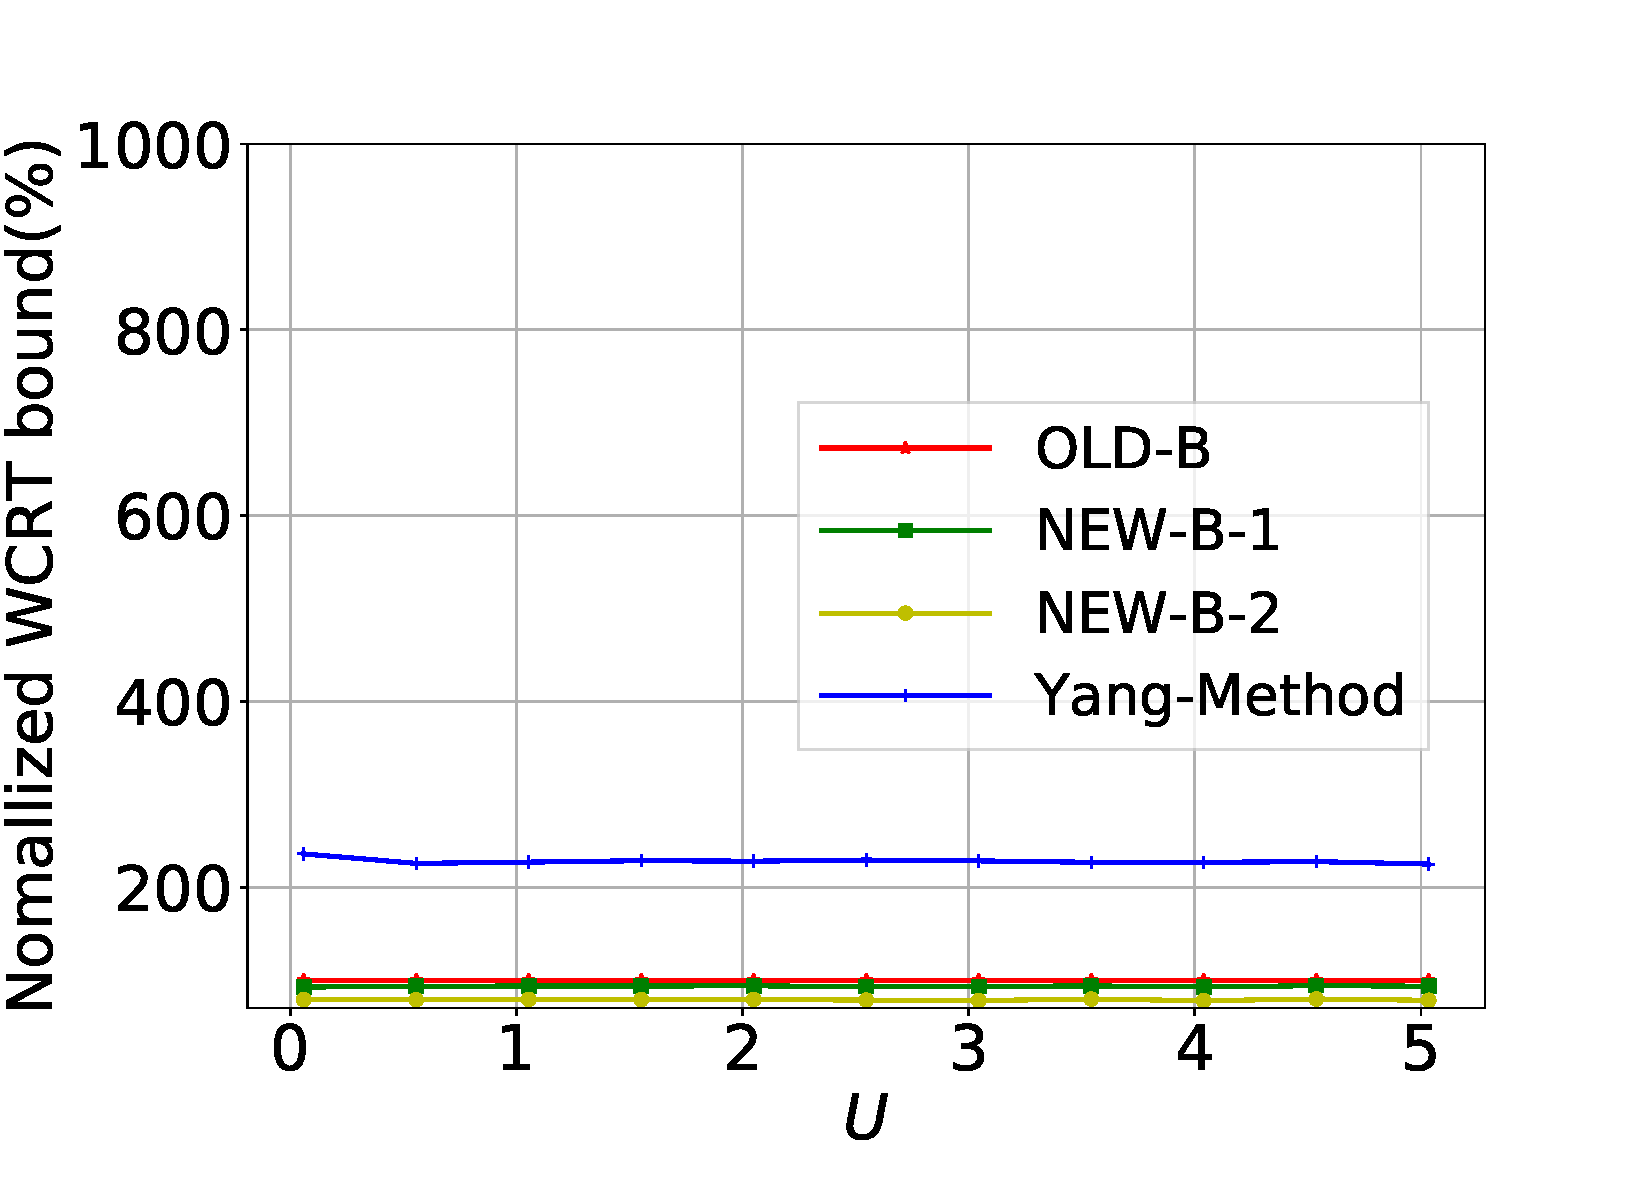
\includegraphics[scale=0.2]{figure/urtr.pdf}}
	\subfigure[Norm. bound with changing $|V|$]{ \label{fig:rtrN} %% label for second subfigure 
		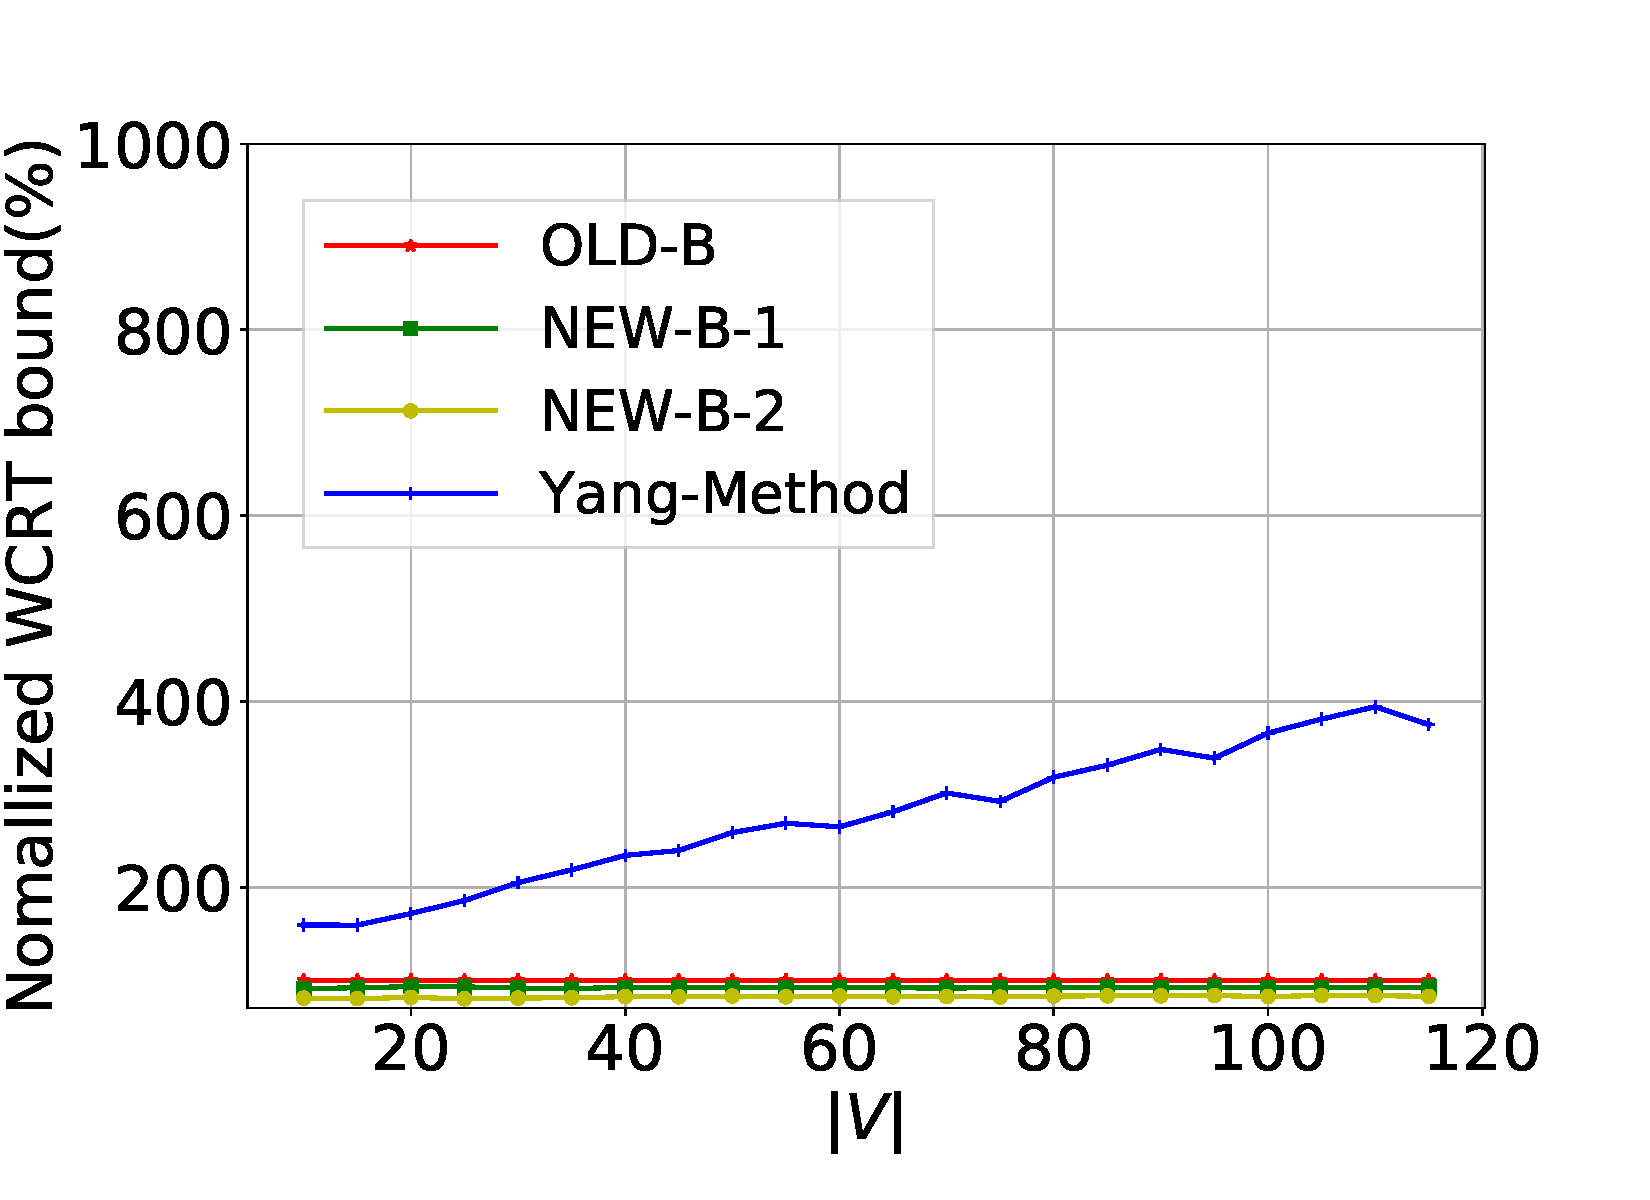
\includegraphics[scale=0.2]{figure/nrtr.pdf}}
	
	\subfigure[Norm. bound with changing $pr$]{  \label{fig:rtrpr} %% label for second subfigure 
		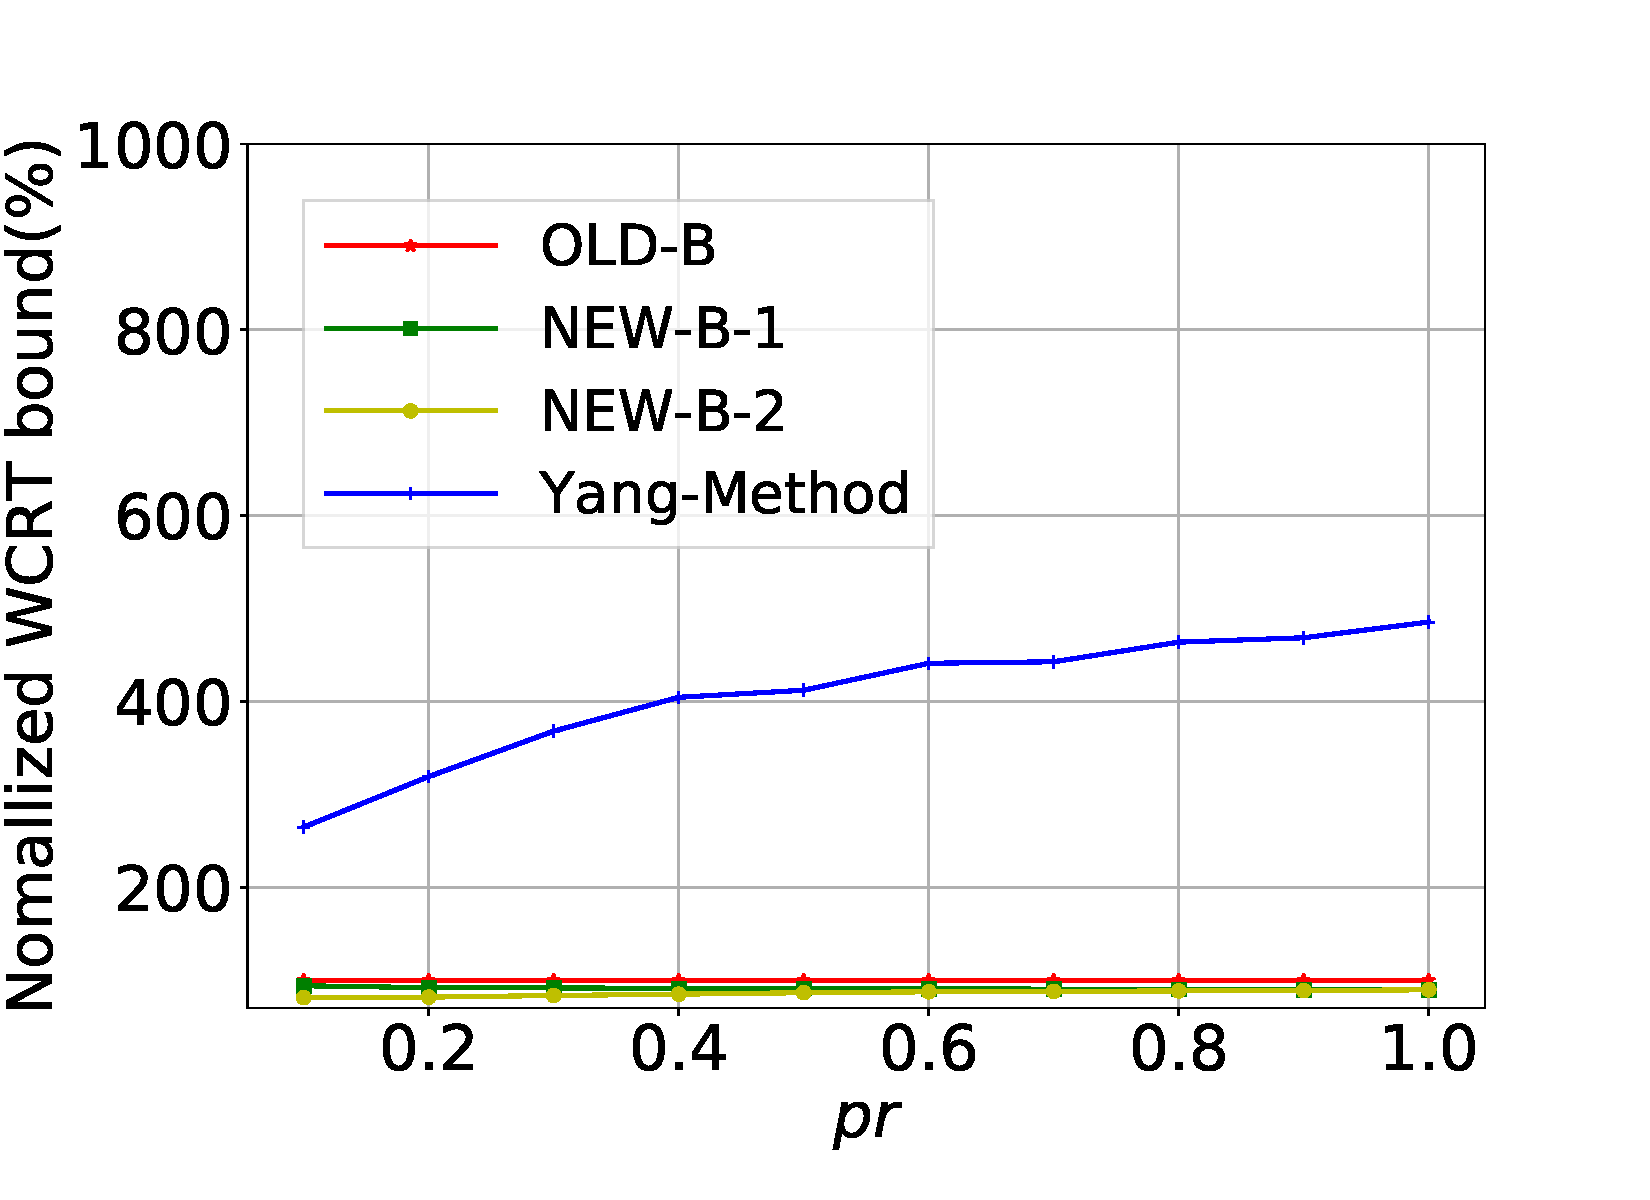
\includegraphics[scale=0.2]{figure/pr.pdf}}
	\subfigure[Norm. bound with changing $|S|$]{ \label{fig:rtrpn}%% label for second subfigure 
		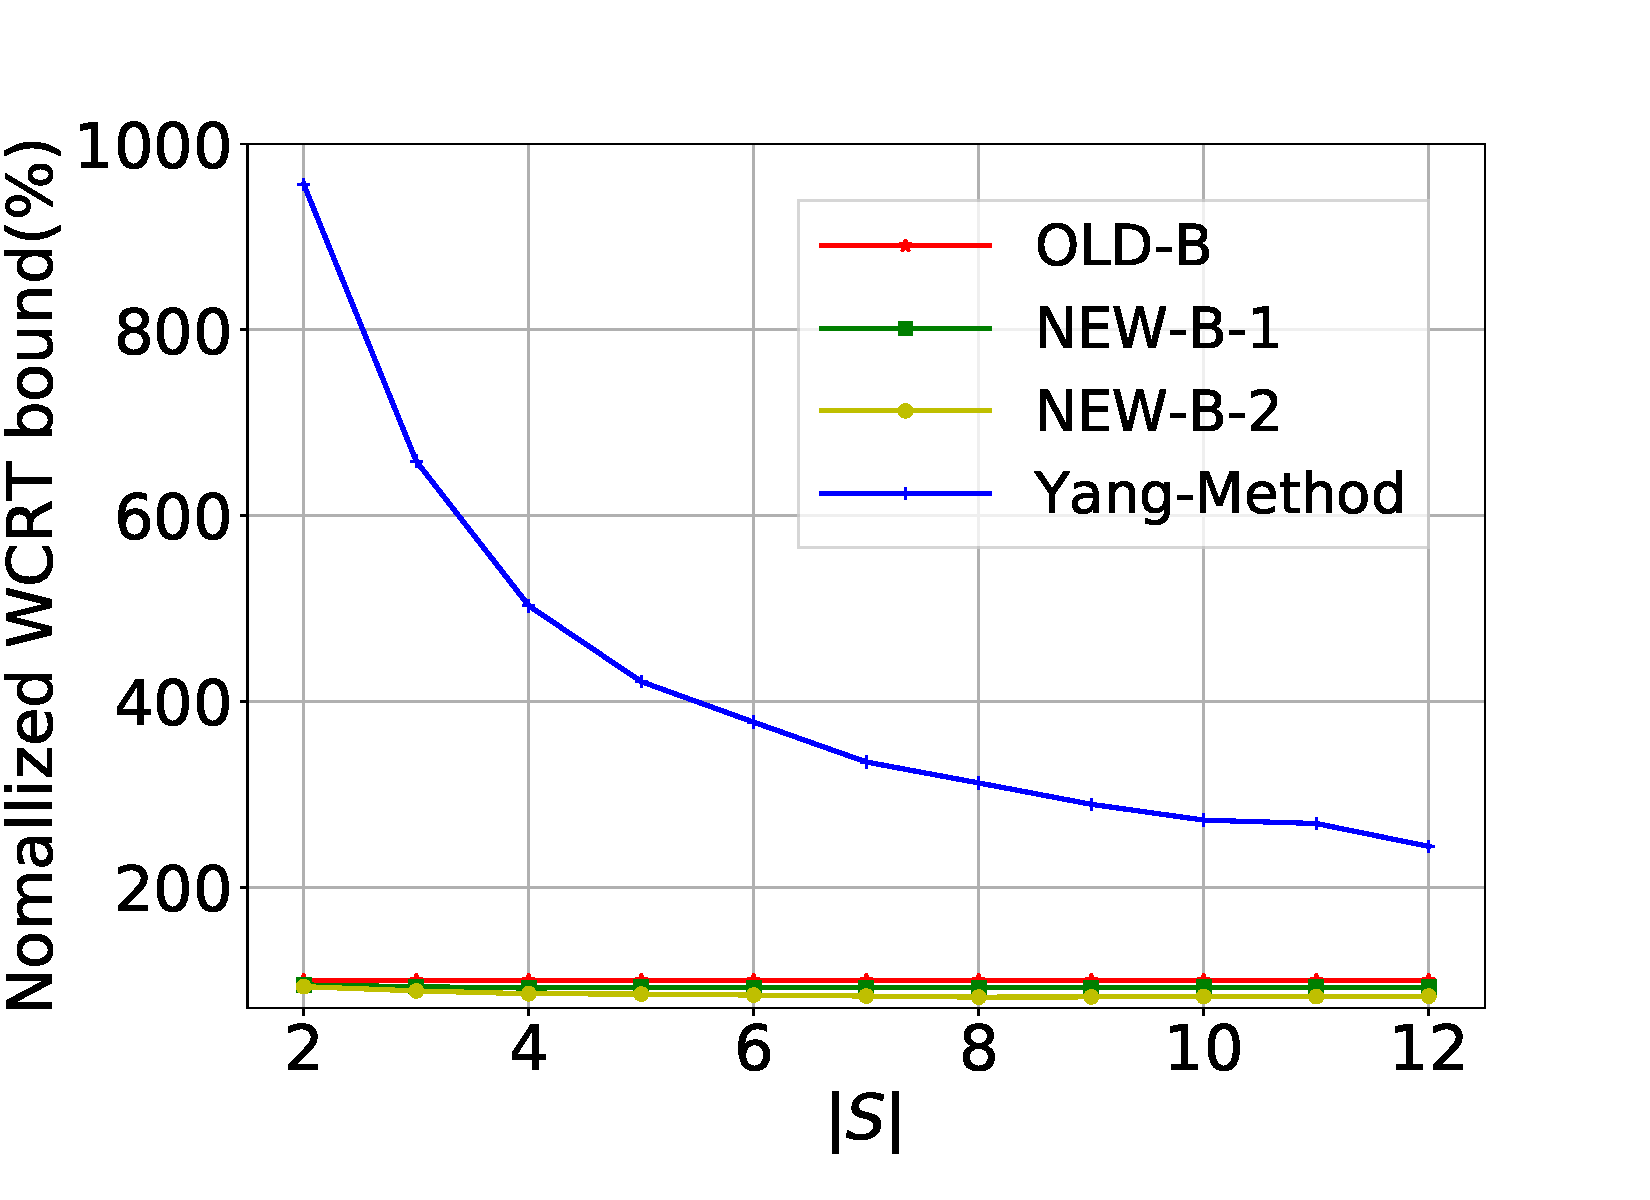
\includegraphics[scale=0.2]{figure/pnrtr.pdf}}	
	
	\caption{Comparison of analysis precision of different bounds.} 
	\label{fig:precise} %% label for entire figure 
\end{figure}

\section{case study}

\begin{figure} 
	\centering  
	\subfigure[$G_1$]{\label{fig:g1} %% label for second subfigure 
		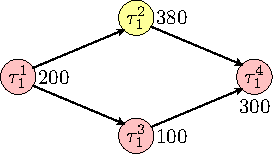
\includegraphics[scale=0.9]{figure/example.pdf}}
	\subfigure[$G_2$]{ \label{fig:g2} %% label for second subfigure 
		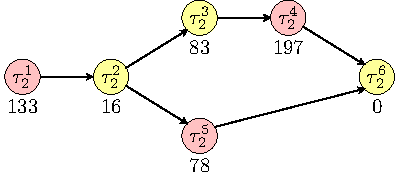
\includegraphics[scale=0.9]{figure/example2.pdf}}
	\subfigure[$G_3$]{  \label{fig:g3} %% label for second subfigure 
		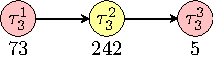
\includegraphics[scale=0.9]{figure/example3.pdf}}	
	
	\caption{DAG tasks in this case study each task with 2 types vertices.} 
	\label{fig:tasks} %% label for entire figure 
\end{figure}



We use 3 examples to show the pessimistic of \textbf{Yang-Method} and these DAG tasks are shown in case study section in \cite{Yang2016}. In Figure \ref{fig:tasks}, there are two types processors: the one filled with red is type 1 and the one filled with yellow is type 2. And we also assume $M_1=M_2=2$.
\begin{example}
	\label{ex:cases1}
	In this DAG task $G_1$, there are four vertices and $T_1=500$. The WCET of each vertex is shown in the Fig.\ref{fig:g1} next to the vertex.
	According to Equation \eqref{eq:rt}, we can get the WCRT of these four vertices as following when we assume the deadline of each vertex is equal with the period.
	
	\[
	\begin{split}
		R_1^1&=\frac{1}{2}\left(500 \times \frac{200+100+300}{500}+\frac{200}{500}(500-500)+\frac{100}{500}(500-500)+\frac{300}{500}(500-500)\right)\\
		&+\max\{200,100,300\}+\frac{2-1}{2}\times 200\\
		&=700
	\end{split}	\]
	
		\[
		\begin{split}
		R_1^2&=\frac{1}{2}\left(500 \times \frac{380}{500}+\frac{380}{500}(500-500)\right)
		+\max\{380\}+\frac{2-1}{2}\times 380\\
		&=760
		\end{split}	\]
		
		
		\[
		\begin{split}
	R_1^3&=\frac{1}{2}\left(500 \times \frac{200+100+300}{500}+\frac{200}{500}(500-500)+\frac{100}{500}(500-500)+\frac{300}{500}(500-500)\right)\\
	&+\max\{200,100,300\}+\frac{2-1}{2}\times 100\\
	&=650
		\end{split}	\]
		
			\[
			\begin{split}
			R_1^4&=\frac{1}{2}\left(500 \times \frac{200+100+300}{500}+\frac{200}{500}(500-500)+\frac{100}{500}(500-500)+\frac{300}{500}(500-500)\right)\\
			&+\max\{200,100,300\}+\frac{2-1}{2}\times 300\\
			&=750
			\end{split}	\]
And according to Equation \eqref{eq:rofs}, we have:
\[
\varphi_1^2=\varphi_1^3=\varphi_1^1+R_1^1=700
\]

\[
\varphi_1^4=\max\{\varphi_1^3+R_1^3,\varphi_1^2+R_1^2\}=1460
\]

According to the Equation \eqref{eq:R}, we have:
\[
R_1=1460+750=2210
\]
When using the LP-based deadline to minimize the maximum end-to-end WCRT of task $G_1$. There are only two paths in $G_1$, such as $\pi_1=\{\tau_1^1,\tau_1^2,\tau_1^4\}$ and $\pi_2=\{\tau_1^1,\tau_1^3,\tau_1^4\}$. According to the Equation \eqref{eq:rofs} and \eqref{eq:R}, we have:

\begin{equation}
\label{eq:lpR}
	R_1=\max\{R_1^1+R_1^2+R_1^4,R_1^1+R_1^3+R_1^4\}
\end{equation}
When $0\leq D_1^1\leq 500$, $0\leq D_1^2\leq 500$, $0\leq D_1^3\leq 500$, $0\leq D_1^4\leq 500$, the purpose is to find the minimum of $R_1$ computed by \eqref{eq:lpR}.

\begin{equation*}
\begin{split}
	R_1^1+R_1^2+R_1^4&=\frac{1}{2}\left(D_1^1 \times \frac{200+100+300}{500} + \frac{200}{500}(500-D_1^1)+ \frac{100}{500}(500-D_1^3)+\frac{300}{500}(500-D_1^4)\right)\\
	&+300+\frac{200}{2}\\
	&+\frac{1}{2}\left(D_1^2 \times \frac{380}{500}+\frac{380}{500}(500-D_2^2)\right)\\
	&+380+\frac{380}{2}\\
	&+\frac{1}{2}\left(D_1^4\times \frac{200+100+300}{500} + \frac{200}{500}(500-D_1^1)+ \frac{100}{500}(500-D_1^3)+ \frac{300}{500}(500-D_1^4)\right)\\
	&+300+\frac{300}{2}\\
	&=700+\frac{1}{2}\left(\frac{4}{5}D_1^1-\frac{1}{5}D_1^3-\frac{3}{5}D_1^4\right)+760\\
	&+750+\frac{1}{2}\left(\frac{3}{5}D_1^4-\frac{1}{5}D_1^3-\frac{2}{5}D_1^1\right)\\
	&=2210+\frac{2}{10}\left(D_1^1-D_1^3\right)
\end{split}
\end{equation*}

Similar we can get:

\begin{equation*}
\begin{split}
	R_1^1+R_1^3+R_1^4&=\frac{1}{2}\left(D_1^1\times \frac{200+100+300}{500} + \frac{200}{500}(500-D_1^1)+ \frac{100}{500}(500-D_1^3)+ \frac{300}{500}(500-D_1^4)\right)\\
	&+300+200/2\\
	&+\frac{1}{2}\left(D_1^3 times \frac{200+100+300}{500} + \frac{200}{500}(500-D_1^1)+ \frac{100}{500}(500-D_1^3)+ \frac{300}{500}(500-D_1^4)\right)\\
	&+300+\frac{2-1}{2}\times 100\\
	&+\frac{1}{2}\left(D_1^4\times \frac{200+100+300}{500} + \frac{200}{500}(500-D_1^1)+ \frac{100}{500}(500-D_1^3)+ \frac{300}{500}(500-D_1^4)\right)\\
	&+300+300/2\\
	&=700+\frac{1}{2}\left(\frac{4}{5}D_1^1-\frac{1}{5}D_1^3-\frac{3}{5}D_1^4\right)\\
	&+650+\frac{1}{2}\left(D_1^3-\frac{2}{5}D_1^2-\frac{3}{5}D_1^4\right)\\
	&+750+\frac{1}{2}\left(\frac{3}{5}D_1^4-\frac{1}{5}D_1^3-\frac{2}{5}D_1^1\right)\\
	&=2160+\frac{3}{10}\left(D_1^3-D_1^4\right)
\end{split}
\end{equation*}

Finally, when $D_1^1=0,D_1^2=500,D_1^3=500,D_1^4=500$, one get the minimum end-to-end WCRT of $G_1$ as $R_1=2110$.

Because the number of types are the same, so the results of OLD-B equals with NEW-B-1, which is computed as following:
\[
R_1=\frac{200+380+300}{2}+\frac{200+380+300+100}{2}=930
\]

And the result of NEW-B-2 is : $R_1=880$

\end{example}



\begin{example}
	\label{ex:cases2}
	In this DAG task $G_2$, there are 6 vertices and $T_2=1000$. The WCET of each vertex is shown in the Fig.\ref{fig:g2} next to the vertex.
	According to Equation \eqref{eq:rt}, we can get the WCRT of these four vertices as following when we assume the deadline of each vertex is equal with the period.
	
	\[
	\begin{split}
	R_2^1&=\frac{1}{2}\left(1000 \times \frac{133+197+78}{1000}+\frac{133}{1000}(1000-1000)+\frac{197}{1000}(1000-1000)+\frac{78}{1000}(1000-1000)\right)\\
	&+\max\{133,197,78\}+\frac{2-1}{2}\times 133\\
	&=467.5
	\end{split}	\]
	
	\[
	\begin{split}
	R_2^2&=\frac{1}{2}\left(1000 \times \frac{16+83}{1000}+\frac{16}{1000}(1000-1000)+\frac{83}{1000}(1000-1000)\right)
	+\max\{16,83\}+\frac{2-1}{2}\times 16\\
	&=140.5
	\end{split}	\]
	
	
	\[
	\begin{split}
	R_2^3&=\frac{1}{2}\left(1000 \times \frac{16+83}{1000}+\frac{16}{1000}(1000-1000)+\frac{83}{1000}(1000-1000)\right)
	+\max\{16,83\}+\frac{2-1}{2}\times 83\\
	&=174
	\end{split}	\]
	
	\[
	\begin{split}
	R_2^4&=\frac{1}{2}\left(1000 \times \frac{133+197+78}{1000}+\frac{133}{1000}(1000-1000)+\frac{197}{1000}(1000-1000)+\frac{78}{1000}(1000-1000)\right)\\
	&+\max\{133,197,78\}+\frac{2-1}{2}\times 197\\
	&=499.5
	\end{split}	\]
	
		\[
		\begin{split}
		R_2^5&=\frac{1}{2}\left(1000 \times \frac{133+197+78}{1000}+\frac{133}{1000}(1000-1000)+\frac{197}{1000}(1000-1000)+\frac{78}{1000}(1000-1000)\right)\\
		&+\max\{133,197,78\}+\frac{2-1}{2}\times 78\\
		&=440
		\end{split}	\]
		
		
	According to the assumption of \cite{Yang2016} $R_2^6=0$, and according to the Equation \eqref{eq:rofs}, we have:
	\[
	\varphi_2^2=0+467.5=467.5,\ \varphi_2^3=\varphi_2^2+R_2^2=608,\ \varphi_2^4=\varphi_2^3+R_2^3=782, \varphi_2^5=\varphi_2^2+R_2^2=608
	\]
	
	\[
	\varphi_2^6=\max\{\varphi_2^4+R_2^4,\varphi_2^5+R_2^5\}=1281.5
	\]
	
	According to the Equation \eqref{eq:R}, we have:
	\[
	R_2=1281.5+0=1281.5
	\]
	When using the LP-based deadline to minimize the maximum end-to-end WCRT of task $G_2$. Then there are only two paths in $G_2$, such as $\pi_1=\{\tau_2^1,\tau_2^2,\tau_2^3,\tau_2^4,\tau_2^6\}$ and $\pi_2=\{\tau_2^1,\tau_2^2,\tau_2^5,\tau_2^6\}$. According to the Equation \eqref{eq:rofs} and \eqref{eq:R}, we have:
	
	\begin{equation}
	\label{eq:lpR2}
	R_2=\max\{R_2^1+R_2^2+R_2^3+R_2^4+R_2^6,R_2^1+R_2^2+R_2^5+R_2^6\}
	\end{equation}
	When $0\leq D_2^1\leq 1000$, $0\leq D_2^2\leq 1000$, $0\leq D_2^3\leq 1000$, $0\leq D_2^4\leq 1000$, $0\leq D_2^5\leq 1000$, the purpose is to find the minimum of $R_2$ computed by \eqref{eq:lpR2}.
	
	\begin{equation*}
		R_2^1+R_2^2+R_2^3+R_2^4+R_2^6=\frac{1}{2}\left(\frac{142}{1000}D_2^1+\frac{14}{1000}D_2^4-\frac{156}{1000}D_2^5
		+\frac{67}{1000}D_2^2-\frac{67}{1000}D_2^3\right)+1281.5
	\end{equation*}
	
	Similar we can get:
	
	\begin{equation*}
			R_2^1+R_2^2+R_2^5+R_2^6=\frac{1}{2}\left(\frac{142}{1000}D_2^1 + \frac{83}{1000}D_2^2 - \frac{83}{1000}D_2^3 
			-\frac{394}{1000}D_2^4-\frac{252}{1000}D_2^5\right)+1048
	\end{equation*}
	
	Finally, when $D_2^1=0,D_2^2=0,D_2^3=1000,D_2^4=0,D_2^5=1000$, one get the minimum end-to-end WCRT of $G_2$ as $R_1=1170$.
	
	Because the number of types are the same, so the results of OLD-B equals with NEW-B-1, which is computed as following:
	\[
	R_2=\frac{133+16+83+197}{2}+\frac{133+16+83+197+78}{2}=468
	\]
	
	And the result of NEW-B-2 is : $R_2=468$
	
\end{example}


\begin{example}
	\label{ex:cases3}
	In this DAG task $G_3$, there are 3 vertices and $T_3=1000$. The WCET of each vertex is shown in the Fig.\ref{fig:g3} next to the vertex.
	According to Equation \eqref{eq:rt}, we can get the WCRT of these 3 vertices as following when we assume the deadline of each vertex is equal with the period.
	
	\[
	\begin{split}
	R_3^1&=\frac{1}{2}\left(1000 \times \frac{73+5}{1000}+\frac{73}{1000}(1000-1000)+\frac{5}{1000}(1000-1000)\right)\\
	&+\max\{73,5\}+\frac{2-1}{2}\times 73\\
	&=148.5
	\end{split}	\]
	
	\[
	\begin{split}
	R_3^2&=\frac{1}{2}\left(1000 \times \frac{242}{1000}+\frac{242}{1000}(1000-1000)\right)+242+\frac{2-1}{2}\times 242\\
	&=484
	\end{split}	\]
	
	
	\[
	\begin{split}
	R_3^3&=\frac{1}{2}\left(1000 \times \frac{73+5}{1000}+\frac{73}{1000}(1000-1000)+\frac{5}{1000}(1000-1000)\right)\\
	&+\max\{73,5\}+\frac{2-1}{2}\times 5\\
	&=114.5
	\end{split}	\]
	
	
	
	
	According to the Equation \eqref{eq:rofs}, we have:
	\[
	\varphi_3^2=0+148.5=148.5,\ \varphi_3^3=\varphi_3^2+R_3^2=632.5
	\]
	
	
	According to the Equation \eqref{eq:R}, we have:
	\[
	R_3=632.5+114.5=747
	\]
	When using the LP-based deadline to minimize the maximum end-to-end WCRT of task $G_3$. There is only one path in $G_3$, such as $\pi_1=\{\tau_3^1,\tau_3^2,\tau_3^3\}$. According to the Equation \eqref{eq:rofs} and \eqref{eq:R}, we have:
	
	\begin{equation}
	\label{eq:lpR3}
	R_3=R_3^1+R_3^2+R_3^3
	\end{equation}
	When $0\leq D_3^1\leq 1000$, $0\leq D_3^2\leq 1000$, $0\leq D_3^3\leq 1000$, the purpose is to find the minimum of $R_3$ computed by \eqref{eq:lpR3}.
	
	\begin{equation*}
			R_3^1+R_3^2+R_3^3=\frac{1}{2}\left(\frac{68}{1000}D_3^3-\frac{68}{1000}D_3^1\right)+747
	\end{equation*}
	
	
	Finally, when $D_3^1=1000,D_3^2=1000,D_3^3=0,D_2^4=0$, one get the minimum end-to-end WCRT of $G_3$ as $R_3=713$.
	
	Because the number of types are the same, so the results of OLD-B equals with NEW-B-1, which is computed as following:
	\[
	R_3=\frac{73+242+5}{2}+\frac{73+5+242}{2}=320
	\]
	
	And the result of NEW-B-2 is : $R_3=320$
	
\end{example}

Summarized the results of these three examples, then we have the following table:

\begin{table}[!htbp]
	\centering
	\caption{Results of 3 examples}\label{tab:tb1}%���ӱ��� ���ñ�ǩ
	\begin{tabular}{c|c|c|c|c}
		\hline
		task & Yang-Method, implicit deadline&  Yang-Method, LP-based deadline&NEW-B-1(OLD-B)&NEW-B-2\\
		\hline
		$G_1$& 2210& 2110&930&880\\
		\hline
		$G_2$& 1281.5& 1170&468&468\\
		\hline
		$G_1$& 747& 713&320&320\\
		\hline
	\end{tabular}
	%\caption{����һ�����߱�}\label{tab:aStrangeTable}  �����������Ҳ�ǿ��Ե�
\end{table}



\bibliographystyle{plain}
\bibliography{bibtypedscheduling}


\end{document}
